
\section{Warm-up questions}

\subsection{Thresholding methods}
\begin{qbox}
Cite different methods in order to find a threshold value to binarize a grayscale image. Explain the Otsu's method. What are its limits?
\end{qbox}

\subsection{Image filtering}
\begin{qbox}
 \begin{itemize}
  \item What is the difference between a rank filter and a linear filter?
  \item Cite the name of a filter of each type.
  \item In case of a salt and pepper noise present in the image, what type of filter would you require to restore it? Why?
  \item For the latter, precise its limits and propose a way to improve the result.
 \end{itemize}

\end{qbox}

\subsection{Retina images}
\begin{qbox}
As a project, you coded a method for retina vessels segmentation. Explain the principles of the algorithm.
\end{qbox}



\section{Open question: QR code}
A QR code is a binary code represented as a 2D matrix. A scanner is in charge of reading it (via a camera) and translating it into the actual code. The structure of a QR code is represented in Fig.\ref{fig:structure}.

\begin{figure}[htbp]
 \centering\caption{Conversion of a binary pattern into a binary matrix.}%
 \subfloat[Structure of a QR code, Wikipedia, author: Bobmath, CC-By-SA]{\includegraphics[width=.9\linewidth]{structure.pdf}}
 
  \subfloat[Code.]{
\begin{tikzpicture}
\draw[ultra thick,fill=black] (0,1) rectangle (1,2);
\draw[ultra thick,fill=black] (0,2) rectangle (1,3);
\draw[ultra thick,fill=black] (1,1) rectangle (2,2);
\draw[ultra thick,fill=black] (2,2) rectangle (3,3);
\draw[ultra thick,fill=black] (1,0) rectangle (3,1);
\end{tikzpicture}}\hspace{1cm}
\subfloat[Matrix.]{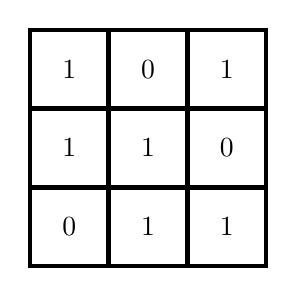
\begin{tikzpicture}
\draw [ultra thick, draw=black] (0,0) grid  (3,3) rectangle (0,0);

\draw (0.5,0.5) node[] {0};
\draw (0.5,1.5) node[] {1};
\draw (0.5,2.5) node[] {1};
\draw (1.5,0.5) node[] {1};
\draw (1.5,1.5) node[] {1};
\draw (1.5,2.5) node[] {0};
\draw (2.5,0.5) node[] {1};
\draw (2.5,1.5) node[] {0};
\draw (2.5,2.5) node[] {1};

\end{tikzpicture}}%
 \label{fig:structure}%
\end{figure}


\begin{qbox}
Describe the different steps required to perform the acquisition and geometric transformation of the QRcode into a binary 2D matrix representing the code (1 value for 1 square, see Fig.\ref{fig:structure}). 
\begin{itemize}
 \item List different situations that may complicate the image acquisition and analysis.
 \item Propose some (image processing) solutions in order to deal with these situations. Explain them, give the necessary details describing the methods.
\end{itemize}

\end{qbox}

\begin{figure}[htbp]
 \centering\caption{Different QR codes. The image acquisition and analysis must be tolerant to different observation conditions... Images from Collectif Raspouteam \url{http://raspouteam.org/}. Other images from unknown sources.}
 \includegraphics[width=.3\linewidth]{orcid_qrcode.png}\hfill
 \includegraphics[width=.3\linewidth]{art.jpeg}\hfill
 \includegraphics[width=.3\linewidth]{image.axd.jpeg}

 \includegraphics[width=.3\linewidth]{paris.jpeg}\hspace{1cm}
 \includegraphics[width=.3\linewidth]{QR_Code_Damaged.jpg}%
\label{fig:qrcodes}%
\end{figure}


